
\chapter{Observable to Study the Underlying Event}

The UE are all the processes not associated with the primary hard scatter in an hadron-hadron collision.

All the process described in the previous section: initial- and final-state radiation, multiple interactions, and beam
remnants and their interactions. These contribute to the Underlying Event (UE) in the proton-proton collision.

The most of the observable to study the UE are sensible only to the sum of these contributions and not to the single ones.

\section{Minimum Bias Measurements and Underlying Event topology}

A Minimum Bias (MB) measurement is a collection of inelastic events with a loose event selection. The event are collected requiring the minimal interaction with the detector (the smallest possible bias). The most of the interaction in MB observation are soft, $p_T\lesssim2\ \mathrm{GeV}$. The study of the UE require at least one hard scattering presence.
 
To study the UE the topological structure of an hadron hadron collision is used. On an event-by-event analysis the direction of the leading object is used to define regions in the $\eta-\phi$ space. Where $\eta$ is the pseudorapidity defined as $\eta=-\log{\tan\left(\frac{\theta}{2}\right)}$, while $\phi$ is the azimuthal angle in the $x-y$ plane. 
The last one is defined from the direction of the leading object as $\Delta\phi=\phi-\phi_{\text{leading}}$ 

\begin{figure}[!ht]
	\centering
	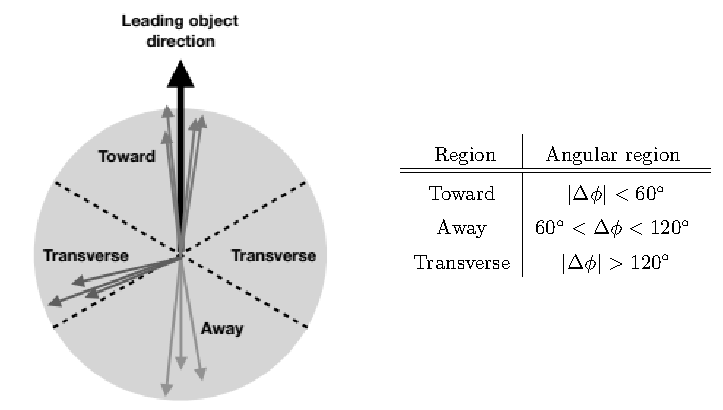
\includegraphics[width=0.8\textwidth]{{img/Regions.pdf}}
	\caption{ADD Caption}
	\label{fig:Regions}
\end{figure}


The regions classification is shown in \figRef{fig:Regions}, we have:
\begin{itemize}
	\item \textbf{Toward region}: the region that contains the leading object, this region contains the most of the particle produced by the hard interaction.
	\item \textbf{Away region}: this region contains the objects that recoil against the leading object, also this region contains mostly the particles produced by the hard interaction.
	\item \textbf{Transverse regions}: the two transverse regions are the most sensitive to UE.
\end{itemize}
The transverse regions are also separated in:
\begin{itemize}
	\item[--] \textbf{TransMAX}: This is the transverse region that contains the \textit{maximum} number of charged particles, or scalar $p_T$ sum of charged particles. This regions includes both MPI and hard-process contamination.
	\item[--] \textbf{TransMIN}: is the transverse region that contains the \textit{minimum} number of charged particles, or scalar $p_T$ sum of charged particles. This region is the most  sensitive to MPI effects.
\end{itemize}



